\documentclass[a4paper]{article}

\input{prelude}

\title{Yanker User Manual}
\author{Antonin Delpeuch}
\date{\today}

\begin{document}

\maketitle

\section{Introduction}

This document describes the \texttt{yanker} software, how to use it, and how
we could improve it.

\section{Purpose}

The categorical framework for compositional and distributional semantics requires
the linguist or the engineer to define different word meaning shapes depending on
the grammatical role of a word.

As a consequence, this framework has not been applied to arbitrary sentence structures,
as it would require the definition of many (hundreds or thousands) different shapes for
the meanings of the words, and probably as many learning strategies for them.

This tool is an attempt to reduce the effort needed to define such shapes. It provides
a graphical editor where the string diagrams corresponding to the word meanings can
be drawn in an intuitive way. Moreover, it allows to define word meanings not only for
particular types, but also for \emph{type skeletons}, i.e. polymorphic types.

\subsection{Type system}

This software currently uses the Lambek calculus as its type system. The Steedman notation
and pregroups should be supported in the near future.

\subsection{Polymorphic types: notation}

We denote type variables by numbers. Hence \texttt{1} should not be confused
with the monoidal unit: it is a variable ranging over all the types. Here are a few examples:
\begin{itemize}
  \item \texttt{N/N} matches only itself (as it contains no variable)
  \item \texttt{1/1} matches any modifier applied to the
        left of the compound it modifies. For instance, it matches \texttt{N/N},
        \texttt{S/S}, \texttt{(N/N)/(N/N)}, but not \texttt{S/N} nor \texttt{N\textbackslash N}.
  \item \texttt{1} matches everything.
  \item \texttt{1/2} matches any type whose root operation is a forward slash.
  \item \texttt{N\textbackslash (S/1)} matches the types \texttt{N\textbackslash(S/N)},
      \texttt{N\textbackslash(S/S)}, \texttt{N\textbackslash(S/(N/N))}, and so on.
\end{itemize}

\section{Tutorial}

\subsection{The graphical interface}

Open Yanker by typing \texttt{yanker} in a terminal. A window opens and it is split vertically
in three areas. From left to right, we have
\begin{enumerate}
  \item The list of type skeletons, i.e. the polymorphic types to which we want to assign
       a string diagram representing the meaning.
  \item The drawing area where we can draw our string diagrams. The string diagram
        currently being displayed corresponds to the skeleton selected in the list on the
        left.
  \item The list of types we would like to cover. By default, this is filled with the
        types occurring in the CCGbank, sorted by decreasing number of occurrences. These
        types have been converted from Steedman notation to Lambek notation.
\end{enumerate}

\begin{figure}[H]
\centering
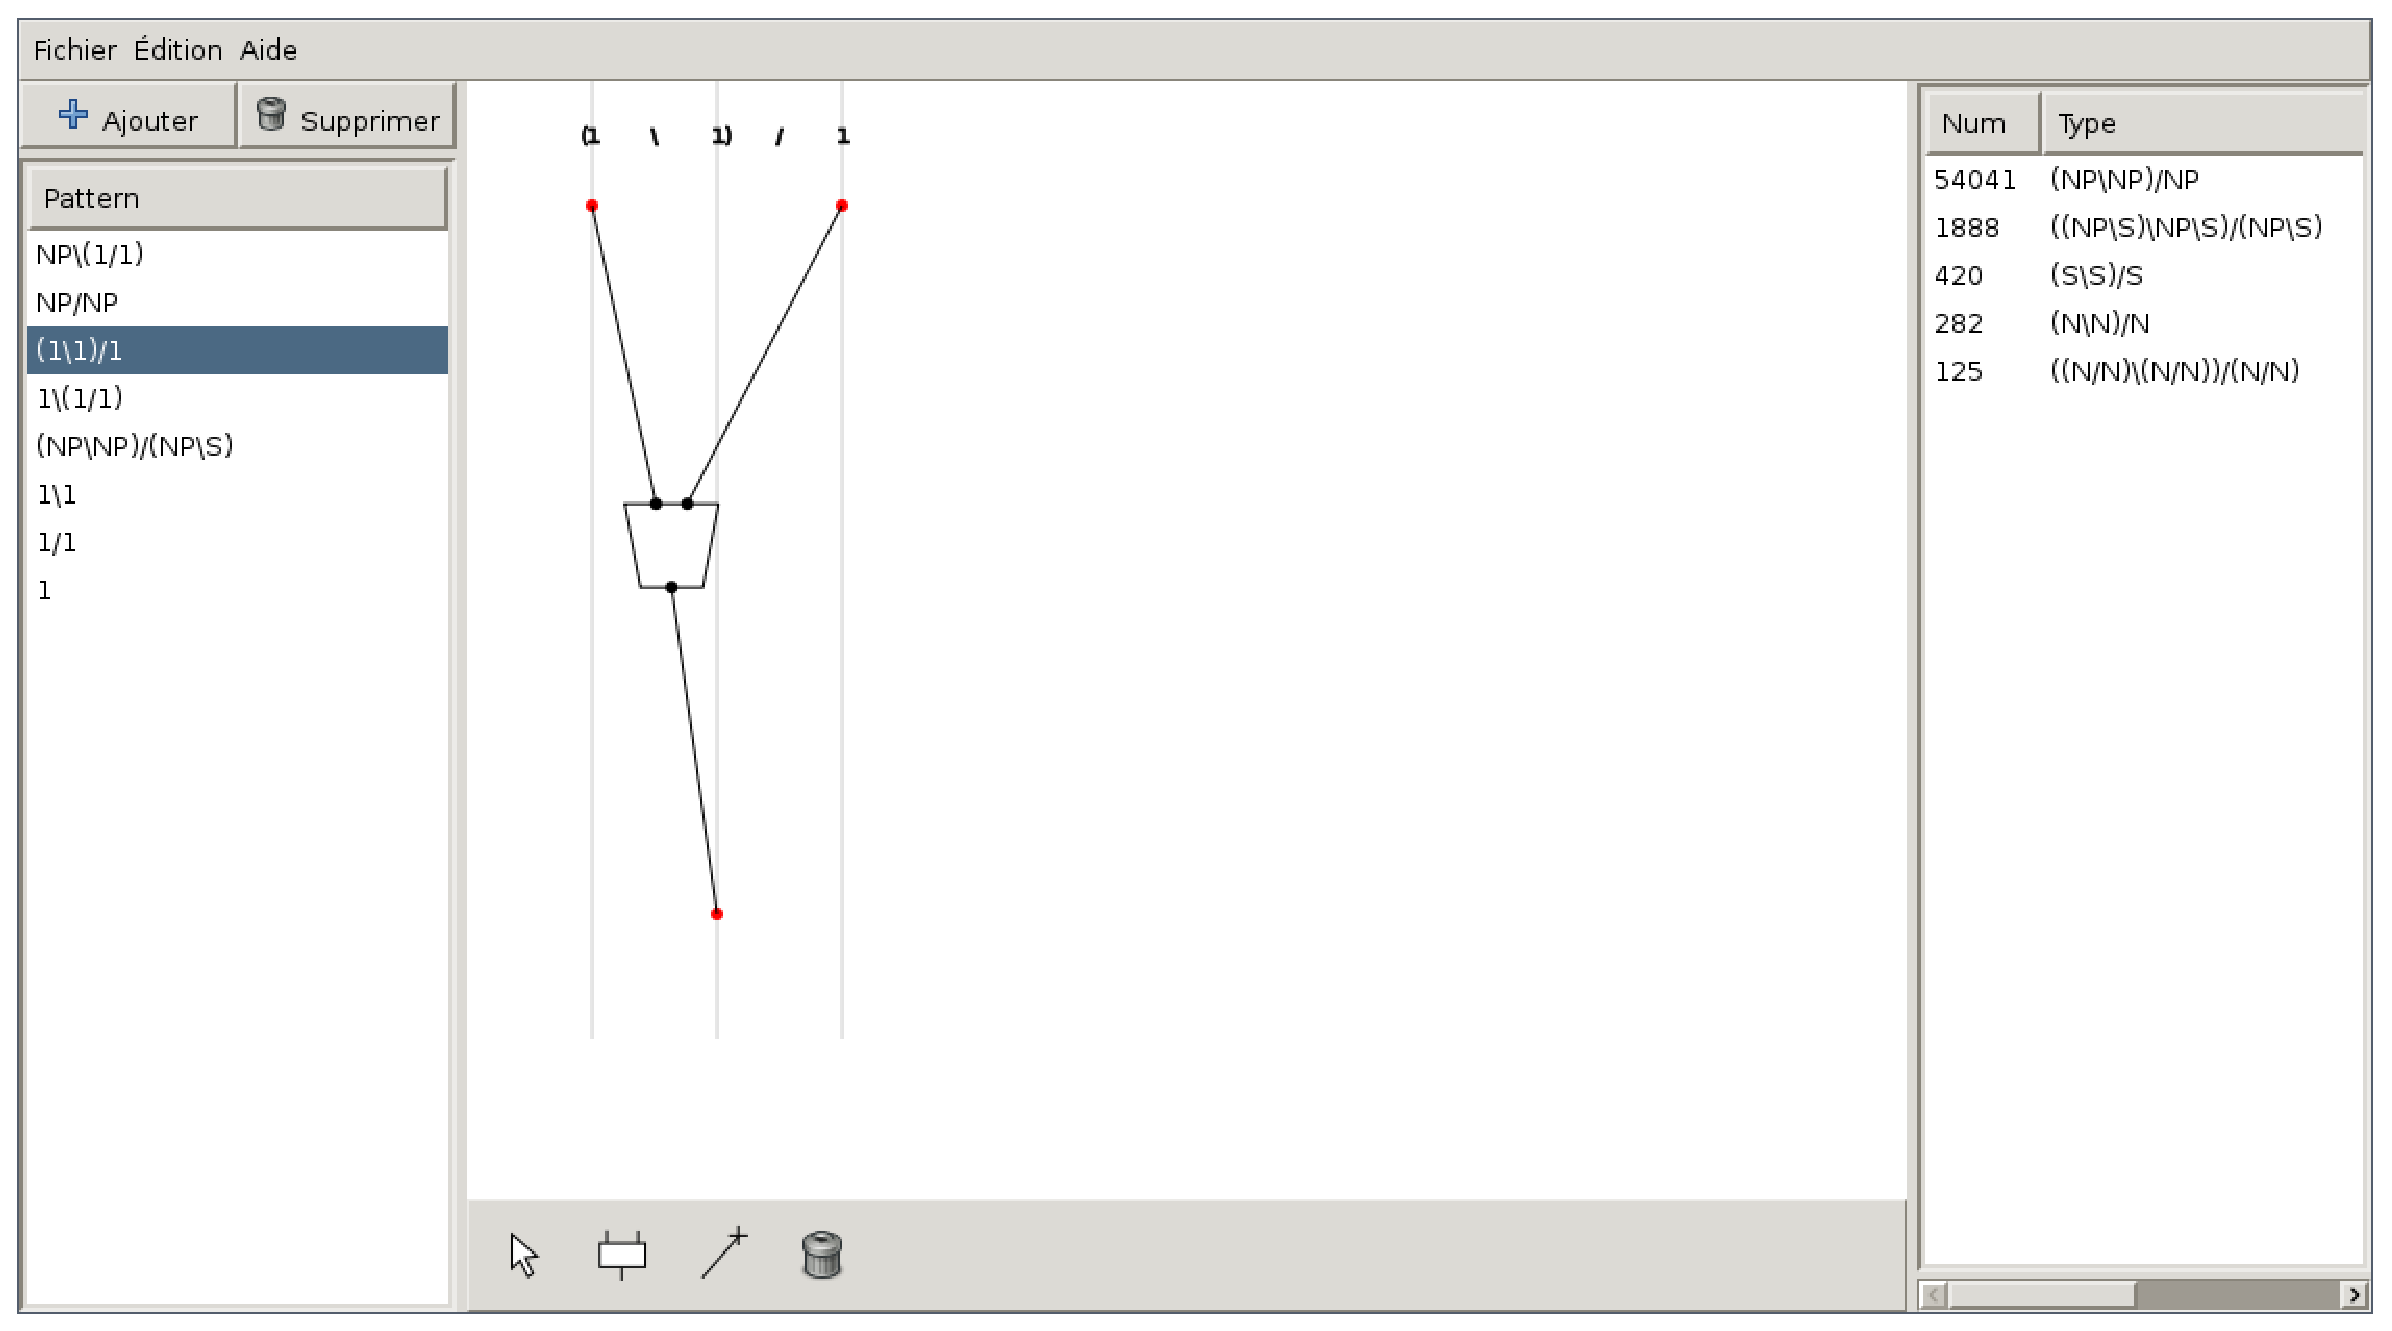
\includegraphics[scale=0.35]{figures/yanker.eps}
\end{figure}

Our goal is that each of these types on the right is matched by a
skeleton eventually, and hence that every type has an associated string diagram.

In the default state, there is only one skeleton, called $1$. Hence it matches
everything. We can give it a default string diagram, which should be simply a vector.
To do so, select the unique type skeleton on the left. Then, click the \emph{New Node}
button, which looks like this:
\includegraphics[scale=0.3]{figures/new\string_node.eps}.

\subsection{Our first diagram}
Move your mouse to the drawing area. You can see that your mouse has grabbed a new node,
that you can put anywhere you want with a click. You should put it above the red dot.
The node has a funny shape: it is because by default, it has neither inputs nor
outputs, hence it acts as a scalar in the category. Using the conventions
introduced by Bob Coecke in analogy to the Dirac notation,
we draw a scalar as a rotated rectangle, or more precisely as two concatenated triangles.

The red dot under our node is a \emph{gate}. As it is drawn at the bottom, it corresponds
to an output. The type associated with this gate is drawn on the same grey line, at the top.
Now we need to connect the node to the gate. To do so, click the \emph{New Edge} button,
which looks like this:
\includegraphics[scale=0.3]{figures/new\string_edge.eps}.
Now, click on the gate, and then on the lower part of
our node. This creates a link between the node and the gate. Horray, we have defined
the meaning of our type skeleton!

\begin{figure}[H]
\centering
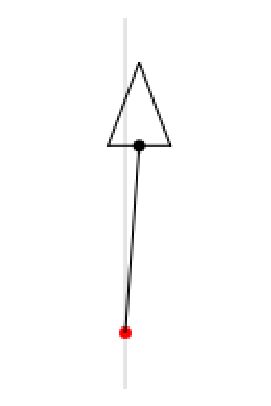
\includegraphics[scale=0.6]{figures/triangle.eps}
\end{figure}

But with this only type skeleton, we have not given any particular structure to word
meanings.

\subsection{More type skeletons}

Let us add a new type skeleton. Click the \emph{Add} button above the skeleton list.
This gives you a text input where you can input a type skeleton, for instance \texttt{1 / 1}.
Confirm the addition.

You will notice that the new type skeleton has been added at the beginning of the list.
The order of that list matters, because the meaning of a type is defined by the
graph associated to the first skeleton it matches. So we want the \emph{1} type skeleton
to be the last one in this list, so that types can match more specific type skeletons.

When you select one of the type skeletons, you will notice that the list of types on
the right changes: the new types are the ones matched by the current type skeleton
(and not matched by any other type skeleton higher up in the list).

\subsection{A default meaning for \texttt{1/1}}

The type skeleton \texttt{1/1} matches any modifier taking its argument to its right,
and as you can see, there are many cases of such words. One simple baseline for all
these modifiers would be to assign the identity as a meaning: with this baseline,
there is nothing to learn, and the information flow is preserved.

Click the \texttt{1/1} skeleton and draw an edge between the gate at the top and
the gate at the bottom. The gate at the top represents the input of our diagram
(where the meaning of the argument comes from) and the gate at the bottom represents
the output (where the meaning of the phrase goes out).

\begin{figure}[H]
\centering
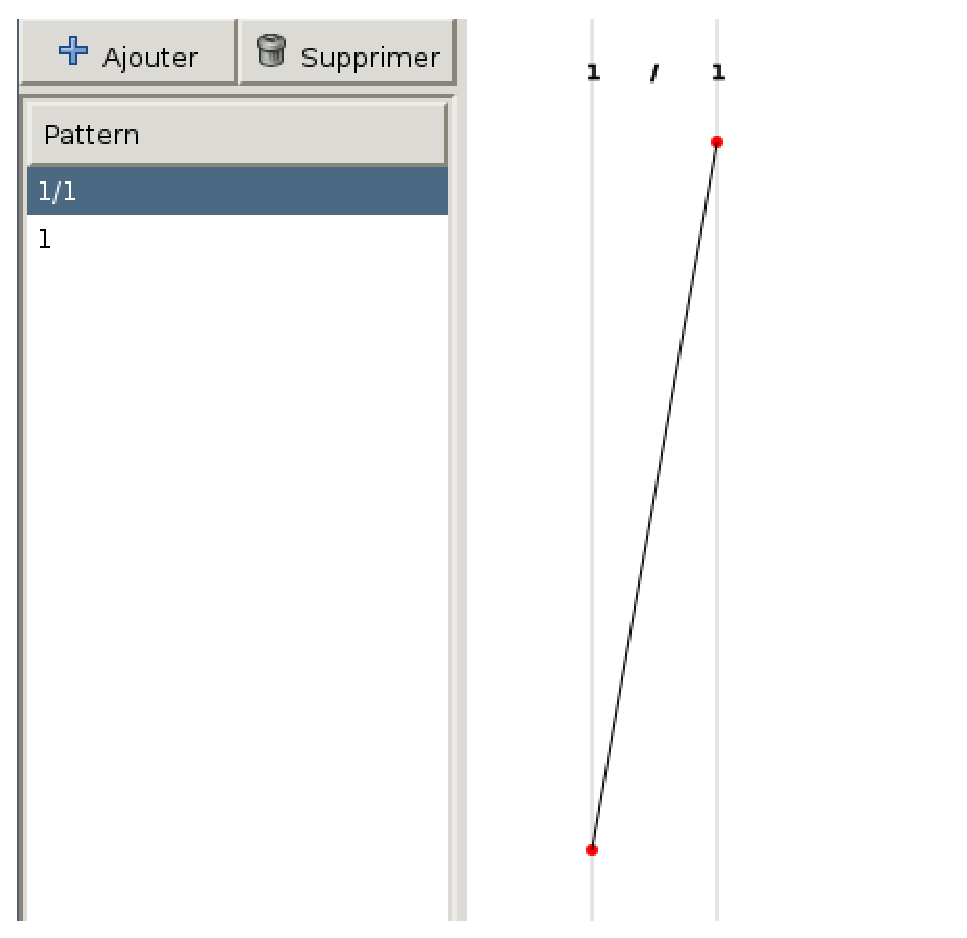
\includegraphics[scale=0.35]{figures/identity.eps}
\end{figure}

For now, this is the end of the tutorial, as we have roughly explored all the
features of this current version. But you can still explore the possiblilities with
other type skeletons and see what types from the CCGbank you get. Not that not all 
the types from the CCGbank appear though, because the current list has been cut for some
reason.

\appendix

\section{Installation}

\subsection{From the source code}
The source code of \texttt{yanker} is available on \url{http://github.com/wetneb/yanker}
and can be retrieved using Git.
It is written in Haskell.
To compile it, the simplest way is probably to use \texttt{cabal}, the standard
build manager for Haskell programs. On Linux, type the following commands in a terminal,
in the directory where the source code was fetched:
\begin{verbatim}
cabal configure
cabal build
\end{verbatim}
It can be installed using the \texttt{cabal install} command. Note that it usually
not necessary to run this command with superuser rights: \texttt{yanker} will be
installed in \texttt{~/.cabal/bin}. Be sure to add this path to your \texttt{\$PATH}
or to type the path in full when you run the program.

\subsection{Using a Debian package}

Debian packages have been compiled for both \texttt{i386} and \texttt{amd64} architectures.
These can be found on the webpage of the program, \url{http://github.com/wetneb/yanker}.


\bibliographystyle{plainnat}
\bibliography{references}

\end{document}

